\subsection{Enable Selector \& Autostart}
\label{sec:ENABLE_AUTOSTART}

\subsubsection{Enable Selector}
\label{sec:ENABLE_SEL}

Taking into account the fact that the 4-digit 7-segment displays receive data from different GALs throughout the different stages of the system, short-circuiting the data lines is very easy. We must therefore prevent this from happening so as to have a functioning system.\medskip

To solve this nuisance, an auxiliary GAL is needed. This device will command the \textit{ENABLE} pins of out custom-designed drivers (See \textbf{Subsubsections \ref{sec:DISPLAY}} \textbf{and} \textbf{\ref{sec:OPEN_MESSAGE}} for more information on this topic). This, in essence avoids short circuits by only having one display driver active at the time (The rest being in High-Z mode).

\medskip

The subsystem has the following inputs: the clock signal (\textit{CLK}), the display signal (\textit{DISP\_EN\_}), which comes from the OPEN/ERROR GALs, and the \textit{READY} signal for the autostart. \medskip

On the other hand, the outputs are: \textit{START}, which commands the beginning of the auto start, and the \textit{DISP\_EN} array that regulates the enable signals of the different sub-circuits.\medskip

As \textit{DISP\_EN\_0} corresponds to the \textbf{\textit{Open}} message, each time that it gets pulled HIGH, the \textit{DISP\_EN1}, which corresponds to the OPEN subcircuit enable signal, must be pulled HIGH too.\medskip

The same principle applies to \textit{DISP\_EN\_1}. This signal corresponds to the \textbf{\textit{Err}} message, so each time that it is pulled HIGH, the \textit{DISP\_EN2}, which corresponds to the ERROR subcircuit enable signal, must be pulled HIGH too.

\medskip

When none of these input signals, i.e. \textit{DISP\_EN\_0} and \textit{DISP\_EN\_1} are HIGH, that means that the display does not have to show neither the \textbf{\textit{Open}} nor the \textbf{\textit{Err}} message, but the password entered by the user. Thus, \textit{DISP\_EN0}, which is the enable for the decoder of the password, must be pulled HIGH.\medskip

\subsubsection{Autostart}
\label{sec:AUTOSTART}

The autostart subsystem, as the name suggests, is in charge of starting the system automatically when the simulation begins. This is needed because the ring counter that we discussed in \textbf{Subsection \ref{sec:KEYPAD}} needs to be pre-loaded in order to start.\medskip

In a real case scenario, a single pulse generator, such a monostable could be used to generate the required pulse. For the simulation though, it is a tad more complex, as the simulation takes some time to load, and non-linear components such as diodes tend to act in a weird way if they are powered before starting it. That is why we cannot simply connect one of the pulse generators that we discussed in \textbf{Section \ref{sec:DELAYED_PULSE}} to the \textit{START} signal and expect it to run flawlessly. \medskip 

\clearpage

To overcome this problem, we have simply delayed the operation of the pulse generator by performing some unnecessary actions. Since we had some pins left in the Enable Selector GAL, we decided to use it to generate said delay. In the code we can see that the GAL reads the value of the \textit{READY} signal, which is HIGH when the simulation starts and it checks that it is indeed HIGH, and as a consequence, it pulls the \textit{TURN\_ON} HIGH. After that, the signal passes through a buffer, so as to add its propagation time to the one of the GAL, and, finally, the pulse generator is triggered, pre-loading the initial ring counter and starting the system.\medskip

This part of the code would not be needed in a real case scenario as its only function is to wait for the simulation to load properly before starting the system. \medskip

The VHDL code that describes this subsystem can be found below:

\inputcode{Code/ENABLES.vhd}

The Proteus Subassembly of both circuits is attached below:

\vspace{-0.5cm}

\begin{figure}[H]
    \centering
    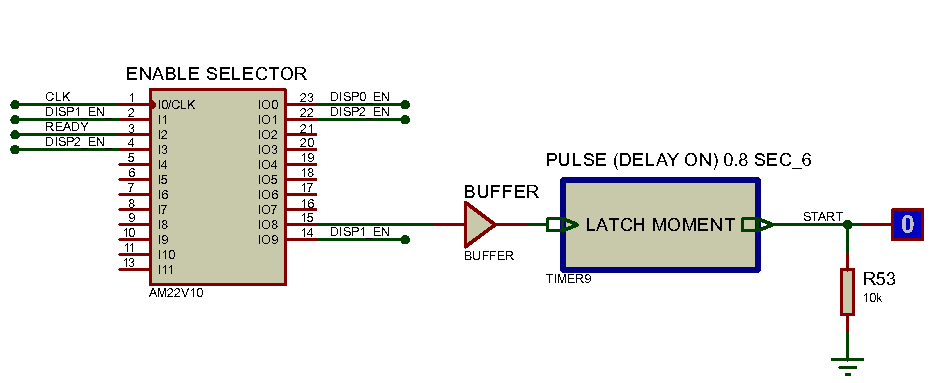
\includegraphics[scale = 0.85]{Graphics/ENABLE SELECTOR + AUTOSTART/ENABLE_SELECTOR_AUTOSTART_PROTEUS.PDF}
    \caption{Enable Selector \& Autostart Proteus Subassembly}
    \label{fig:my_label}
\end{figure}{}
